\documentclass[tikz,border=2pt]{standalone}
\usepackage{amsmath,amssymb}
\usepackage{pgfplots}
\pgfplotsset{compat=1.18}
\usetikzlibrary{arrows.meta}
\begin{document}
% Maximum premium P^+ for exponential utility u(x) = -e^{-0.1 x}, loss 0 or 10 with probability 1/2:
% the chord midpoint gives E[u(w-X)]; the wealth with the same utility is w - P^+ with P^+ = 6.20 > E[X] = 5.
% A risk-neutral insurer has P^- = 5, so premiums in [5, 6.20] are acceptable to both. (Plotted with w = 10.)
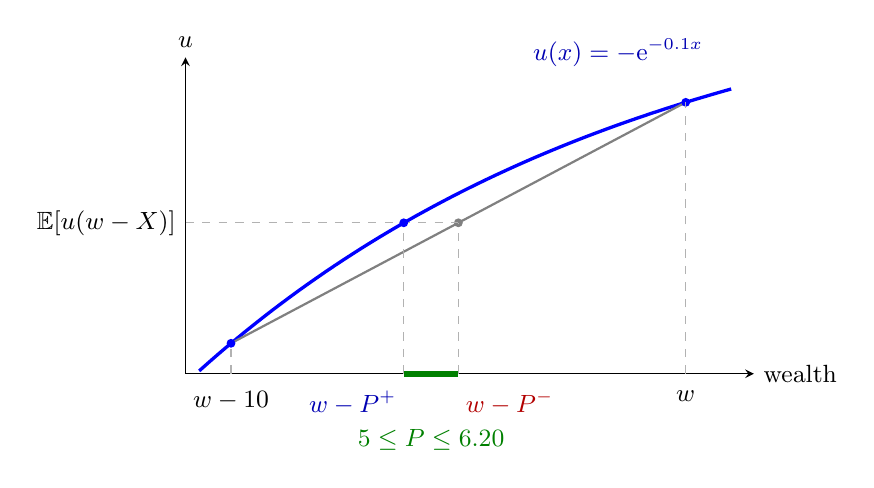
\begin{tikzpicture}[font=\small, >={Latex[length=2mm]}]
  \begin{axis}[
    axis lines=left, xmin=-1, xmax=11.5, ymin=-1.08, ymax=-0.25,
    xtick=\empty, ytick=\empty,
    xlabel={wealth}, ylabel={$u$},
    xlabel style={at={(axis description cs:1,0)}, anchor=west},
    ylabel style={rotate=-90, at={(axis description cs:0,1)}, anchor=south},
    width=8.8cm, height=5.6cm, clip=false
    ]
    \addplot[blue, very thick, domain=-0.7:11, samples=60] {-exp(-0.1*x)};
    \draw[gray, thick] (axis cs:0,-1) -- (axis cs:10,-0.36788);
    \fill[blue] (axis cs:0,-1) circle (1.6pt);
    \fill[blue] (axis cs:10,-0.36788) circle (1.6pt);
    \fill[gray] (axis cs:5,-0.68394) circle (1.6pt);
    \draw[gray!60, thin, dashed] (axis cs:-1,-0.68394) -- (axis cs:5,-0.68394);
    \draw[gray!60, thin, dashed] (axis cs:5,-1.08) -- (axis cs:5,-0.68394);
    \draw[gray!60, thin, dashed] (axis cs:3.7985,-1.08) -- (axis cs:3.7985,-0.68394);
    \draw[gray!60, thin, dashed] (axis cs:0,-1.08) -- (axis cs:0,-1);
    \draw[gray!60, thin, dashed] (axis cs:10,-1.08) -- (axis cs:10,-0.36788);
    \fill[blue] (axis cs:3.7985,-0.68394) circle (1.6pt);
    \draw[green!50!black, line width=2.2pt] (axis cs:3.7985,-1.08) -- (axis cs:5,-1.08);
    % manual tick labels
    \node[anchor=north] at (axis cs:0,-1.1) {$w-10$};
    \node[anchor=north] at (axis cs:10,-1.1) {$w$};
    \node[anchor=north west, red!70!black] at (axis cs:4.95,-1.1) {$w-P^-$};
    \node[anchor=north east, blue!70!black] at (axis cs:3.85,-1.1) {$w-P^+$};
    \node[anchor=east] at (axis cs:-1,-0.68394) {$\mathbb{E}[u(w-X)]$};
    \node[blue!70!black, anchor=south east] at (axis cs:10.6,-0.30) {$u(x)=-\mathrm{e}^{-0.1x}$};
    \node[green!50!black, anchor=north] at (axis cs:4.4,-1.2) {$5\le P\le 6.20$};
  \end{axis}
\end{tikzpicture}
\end{document}
